\section{Results} \label{sec:results}

\subsection{Gene duplication facilitates adaptive evolution of complex traits}

\begin{figure}[!h]
  \centering
  \begin{adjustbox}{scale=0.8}
    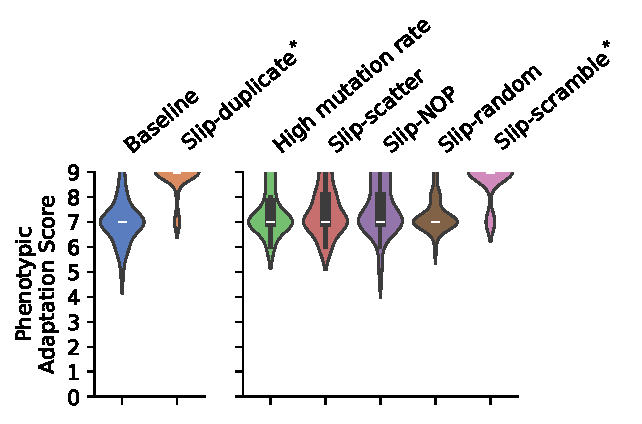
\includegraphics[
        height=4in,
        trim={0.2cm -1.5cm 0.2cm 0},
        clip
      ]{binder/binder/teeplots/col=split+env=static+hue=treatment+inner=box+kind=violin+palette=muted+viz=catplot+x=treatment+y=tasks-present+ext=.pdf}%
    \hspace*{-2.0cm}%
    \raisebox{0.125in}{%
      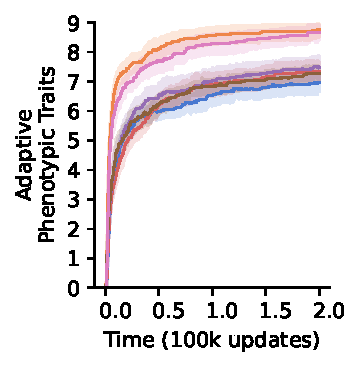
\includegraphics[
          height=2.7in,
          trim={1.36cm -0.64cm 0 0},
          clip
        ]{binder/binder/teeplots/env=static+errorbar=ci+hue=treatment+kind=line+palette=muted+viz=relplot+x=time-100k+y=tasks-present+ext=.pdf}}%
  \end{adjustbox}

  \vspace{-7ex}

  \begin{subfigure}{0.3\textwidth}
    \caption{\small slip-duplication}
    \label{fig:results_panels:slip_duplication}
  \end{subfigure}%
  \begin{subfigure}{0.35\textwidth}
    \caption{\small ablation treatments}
    \label{fig:results_panels:ablation}
  \end{subfigure}%
  \begin{subfigure}{0.22\textwidth}
    \caption{\small lineage history}
    \label{fig:results_panels:time_series}
  \end{subfigure}

  \vspace{1ex}

  \caption{\textbf{Treatments preserving slip-duplicated content facilitate adaptive evolution.}
    \small Violin plots show number of adaptive traits evolved in final dominant genotypes.
    Time series (\ref{fig:results_panels:time_series} right) shows progression of adaptive phenotypic trait counts along lineages of final dominant genotypes; color-coding corresponds to violin plots.
    Asterisk (*) markers indicate treatments with significantly more adaptive phenotypic traits compared to baseline, comparison across both \ref{fig:results_panels:slip_duplication} and \ref{fig:results_panels:ablation} panels.
    Simulation time unit is “updates,” corresponding to evaluation of ~30 genome sites per organism.}
  \label{fig:results_panels}
\end{figure}


In a first set of experiments, we investigated the impact of slip duplications on \textit{de novo} evolution of adaptive phenotypic traits.
We found slip duplications to yield significantly higher evolved trait counts than the baseline treatment (two-tailed Mann-Whitney U test, $W = 562.5$, Bonferroni-adjusted $p << 0.0001$; Figure \ref{fig:results_panels:slip_duplication}).
Many replicates evolved larger genomes, some increasing 10-fold over their original 100-instruction starting point.
To test whether this increased genome length was responsible for adaptive benefits seen in the slip-duplication treatment, we performed additional experiments incorporating a ``long-genome'' control treatment initialized using genomes extended to 1,000 sites by padding the genome with ``no-operation'' instructions that perform no computation (so-called ``NOP'' instructions).

\begin{figure*}
    \centering
    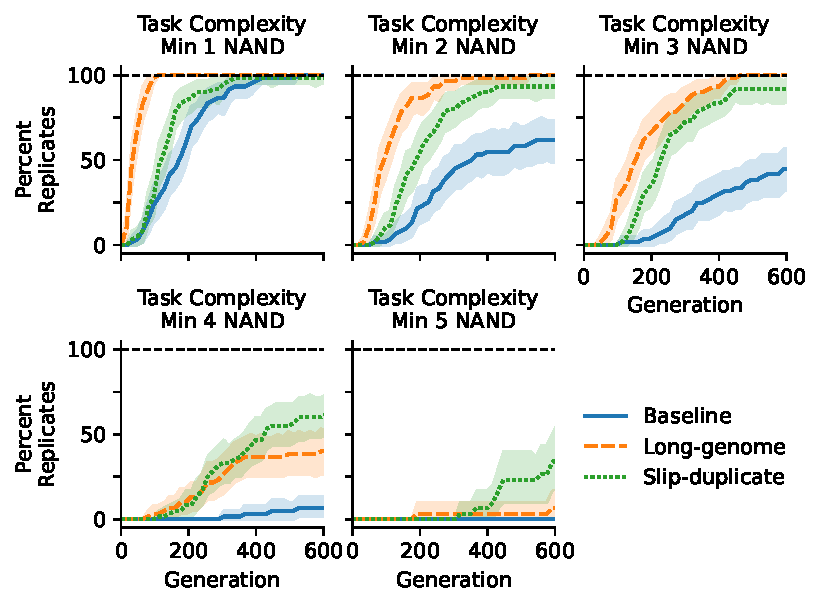
\includegraphics[width=\linewidth]{binder/binder/teeplots/adaptive-evolution-rate.ipynb/col=task-complexity+errorbar=ci+hue=treatment+kind=line+mutation=per site+post=plt-xlim-0-600+style=treatment+viz=relplot+x=generation+y=has-task+ext=.pdf}
    \caption{
        \textbf{Gene duplication boosts adaptive evolution of complex phenotypic traits.}
        \footnotesize
        Plots show fraction of replicates exhibiting available phenotypic traits, by generation from founding ancestor.
        Panels facet by trait complexity, measured by the minimum number of NAND operations required to complete the task.
        Simple tasks (top left) require only one NAND operation.
        More complex tasks (bottom right) require up to five NAND operations as shown in Figure \ref{fig:slip_mut_variants}.
        Slip-duplication treatment facilitates significantly faster adaptive evolution than long-genome treatment for the more complex tasks that require 4 or 5 subcomponents.
        Error bands give 95\% CI, bootstrapped over 30 replicates per treatment.
    }
    \label{fig:adaptive-evolution-rate}
\end{figure*}


We observed that longer genomes evolved significantly greater task acquisition than the baseline genome lengths.
Disaggregating by task complexity, though, reveals impact of genome length as most prominent in the acquisition of simple tasks.
The long-genome control matched or exceeded the performance of slip-duplication in evolving simple traits with 3 or fewer components (Figure \ref{fig:adaptive-evolution-rate}).
% https://github.com/chaynes2019/AvidaGeneDupe/blob/538ede79c7301f10718ca96c8dd38782b6882632/binder/adaptive-evolution-rate.ipynb
However, slip duplication evolved more complex 4- and 5-component traits within a significantly higher fraction of replicates compared to the long-genome control (Fisher's exact tests; 36/60 vs. 24/60, $p<0.05$ [4 components]; 10/30 vs. 2/30, $p<0.03$ [5 components]; Figure \ref{fig:adaptive-evolution-rate}).

% ---
% @AML: Moved to discussion
% These results align with existing findings across a wide variety of biological taxa and digital models that slip-duplication of genetic material can facilitate evolution of adaptive traits \citep{Koza:1995fr,Zhang:2003fw,Teichmann:2004cz}.
% Indeed, a striking example of gene duplication leading to new adaptations comes from the Long-Term Evolution Experiment in \textit{Escherichia coli}, where a duplication in one population broadened expression of key metabolic machinery to previously inhibitive conditions --- resulting in a 7-fold increase in population size \citep{blount_genomic_2012}.
% Among many other examples, such observations motivate longstanding connections drawn between gene duplications and adaptive traits, which date as far back as Ohno \citep{ohno1970evolution}.
% Here, systematic and controlled experimental evidence provides valuable corroboration for this understanding --- and, additionally, suggests in further detail that gene duplications may be especially important to the evolution of complex traits.
% ---

\subsection{Information content of duplications provides adaptive benefit}

Having observed that slip-duplicate mutations accelerate evolution of adaptive phenotypic traits, we next sought to isolate the aspects of slip duplication contributing to adaptation.
For this purpose, we tested four variants of the slip-duplication operator, disabling or replacing a particular aspect of slip duplication (overviewed in Figure \ref{fig:slip_mut_variants}), as well as an additional ``high mutation rate'' treatment where single-site insertion/deletion mutations were applied in lieu of slip mutation.

As shown in Figure \ref{fig:results_panels}, we detected benefits to adaptive evolution only for the follow-up slip-scramble treatment --- which randomized sequence order within duplicated regions (two-tailed Mann-Whitney U test; \Cref{fig:results_panels:slip_duplication,fig:results_panels:ablation}).
All other slip-duplicate variants were indistinguishable or slower-adapting compared with the baseline treatment.

% ----
% @AML: Moved to discussion
% Interestingly, unlike our long-genome control, we did not observe an adaptive benefit from the nop-insert slip-duplication treatment.
% One possible explanation for this difference is the long-genome control's inability to rapidly shrink genome size through slip deletions.
% Indeed, in preliminary experiments we found that deleterious mutational load associated with larger genome size frequently drove genome shrinkage, necessitating enforcement of a lower bound on genome size.
% This pattern aligns with established theory that contingent factors play an important role in ensuring preservation of new genome content \citep{Innan2010,Wagner1998,Tautz1992}.
% ----

Given the efficacy of the slip-scramble treatment in facilitating adaptation, we additionally tested whether phenotypic adaptation differed between the slip-scramble and full-fledged slip-duplicate operators.
To prevent issues with multiple comparisons, we ran 100 new trials under both treatments for this test.
% p = 0.011
We found that the slip-duplicate treatment did, in fact, yield higher task counts compared to the slip-scramble treatment (two-tailed Mann-Whitney U test, $W = 4305$ respectively, Bonferroni-adjusted $p < 0.02$).
As shown in Supplementary Figure~\ref{fig:ablation-site-counts}, full slip-duplication was also associated with significantly larger genome size compared to the slip-scramble treatment (252 $\pm$ SD 105 vs. 491 $\pm$ SD 223 sites; two-tailed Mann-Whitney U test, $U = 734$, $p < 0.001$).

% @AML: Moved next line into discussion
% These results indicate that both the content and structure of duplicated genetic material contribute to facilitating adaptive evolution.

% As above, earlier-reported experiments within our study system concur with present work, finding sequence content and order to both also benefit adaptive evolution within changing environments \citep{lalejini2017gene}.

% \subsection{How Does Slip Duplication Facilitate Adaptive Evolution?}

% Thus far, we have established that slip-duplications of genetic material can significantly benefit adaptive evolution, and that sequence content and order both contribute to this effect.
% We next sought to explain \textit{how} the structural characteristics of slip duplications promote adaptive evolution in our study system.

% In these investigations, we evaluated three hypotheses around evolutionary dynamics of slip duplications.
% First, we explored how the facilitation of adaptive evolution by gene duplication differed between simple and complex traits promoted by gene duplication.
% Second, we tested for signatures of evolutionary potentiation by gene duplications along lineage histories.
% Finally, we examined how slip duplication influences genetic architecture with respect to brittleness and vestigial genetic material.

\subsection{Duplicated sites are potentiated for complex tasks}

% https://github.com/chaynes2019/AvidaGeneDupe/blob/4c7fa27229094adcb5bdb0b1aec541d0014b0fed/binder/hard-task-gain.ipynb
%             H-statistic       p-value
% Components
% 1              1.011820  3.144672e-01
% 2             22.787798  1.809107e-06
% 3             33.846753  5.962854e-09
% 4             15.359894  8.885441e-05
% 5              9.097744  2.559249e-03
%    Components  Prev Slip Insertion Cumulative Count      mean       std
% 0           1                                 False  0.932088  0.455109
% 1           1                                  True  1.002025  1.164197
% 2           2                                 False  0.588566  0.618479
% 3           2                                  True  1.579974  1.191681
% 4           3                                 False  0.491481  0.700256
% 5           3                                  True  1.516115  0.911430
% 6           4                                 False  0.703793  0.980105
% 7           4                                  True  1.229158  0.654042
% 8           5                                 False  0.583674  0.927917
% 9           5                                  True  1.249985  0.531423
%    Components  Prev Slip Insertion Cumulative Count  size
% 0           1                                 False    60
% 1           1                                  True    48
% 2           2                                 False    60
% 3           2                                  True    56
% 4           3                                 False    60
% 5           3                                  True    59
% 6           4                                 False    52
% 7           4                                  True    52
% 8           5                                 False    20
% 9           5                                  True    20

\begin{figure}
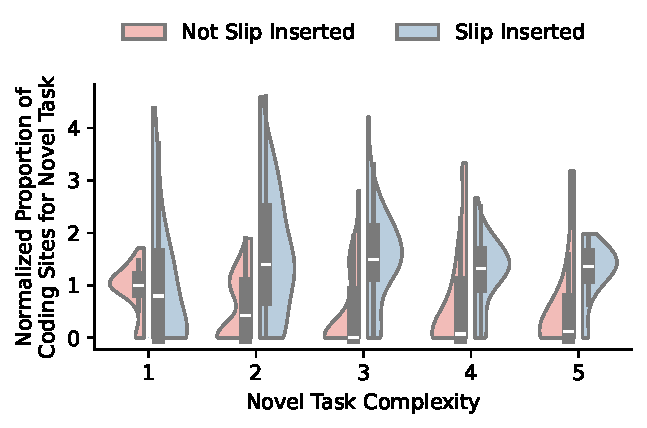
\includegraphics[
width=\linewidth
]{binder/binder/teeplots/density-norm=width+hue=prev-slip-insertion-cumulative-count+kind=violin+viz=catplot+x=components+y=is-task-coding-site+ext=.pdf}
\caption{%
  \textbf{Slip-duplicated sites are overrepresented among \textit{de novo} coding sites for complex traits.}
  \footnotesize
  Distributions compare frequencies of previously slip-duplicated and non-slip-duplicated sites among  \textit{de novo} task coding sites, normalized to neutral expectation.
  Values greater than 1 indicate that sites are overrepresented among the coding sites of novel traits compared to their background frequency.
  Differences between slip-duplicated and non slip-duplicated sites are significant for tasks requiring 2 or more NAND components (Mann-Whitney test; $p < 0.01$).
} \label{fig:potentiation}
\end{figure}


Thus far, we have established that slip duplication can promote evolution of novel traits, with this effect biasing toward complex traits.
% We next sought to characterize aspects of genetic architecture through which slip duplication drives adaptation.
We next sought to understand whether duplicated genetic material itself exhibits elevated potential to code for novel traits.

To address the question, we assessed the density of coding sites for novel adaptive traits in genome regions that had previously been slip duplicated.
Coding sites for these traits arising more frequently than expected by chance in duplicated regions would suggest that these regions are ``potentiated'' --- that is, possessing latent gene content prone to facilitate new traits.
Figure \ref{fig:potentiation} compares the involvement of sites having undergone slip duplication --- versus those that had not --- in coding for novel traits.
For the simplest tasks, requiring only one NAND component, we found no significant difference in the likelihood of duplicated sites participating in coding regions for new tasks.
% https://github.com/chaynes2019/AvidaGeneDupe/blob/2d31c0bd0cc9bdbf4bb49224859d6bd165cd36c8/binder/hard-task-gain2.ipynb
However, we found significant associations for traits with two or more NAND components (one-sample Wilcoxon signed-rank tests; $n=56,59,52,20$ observations).
Effect sizes on probability to code for novel traits were $1.6\times$, $1.6\times$, $1.2\times$, and $1.2\times$, respectively, for 2, 3, 4, and 5 task components.
Smaller effect sizes at 4- and 5-component tasks may be due to a larger portion of the genome becoming comprised of slip-duplicated sites (Supplementary Figure \ref{fig:potentiation-supp}).

One possible confounding factor in coding site analysis is mutational sensitivity at genome sites involved in organisms' self-replication loops.
These sites are critical to viability, with lethal outcomes when knocked out.
We found that these critical sites were indeed less likely to be involved in slip duplication and also less likely to be involved in coding for \textit{de novo} traits.
% Hence, a spurious correlation could be introduced.
After excluding fitness-critical sites from analysis, though, we still found generally similar potentiation signatures from slip duplication (Supplemental Figure \ref{fig:potentiation-supp}).

In addition to potentiating effects, gene duplications are also hypothesized to directly facilitate adaptation, for example, by altering gene product dosage \citep{kondrashov2012gene}.
% https://github.com/chaynes2019/AvidaGeneDupe/blob/61ea29d989ebc8ad83dcfee94f3fa556b81e3f78/binder/gain-mechanism.ipynb
In line with this possibility, we observed that a substantial fraction of novel gain-of-function steps on lineages coincided with slip duplications --- 41 of 174, or 23.6\%.
However, in these cases where slip duplication produced immediate gain-of-function, we still found evidence that sites coding for a new trait were more likely than chance to have been involved in earlier slip duplications (Supplemental Figure \ref{fig:potentiation-supp}).
% @AML, moved the line below to the discussion
% Thus, the adaptive characteristics of slip duplication observed in our system seem likely to result from a combination of potentiation and direct facilitation.

\subsection{Genome length drives genetic complexity}

\begin{figure}
    \centering
    \begin{subfigure}{\linewidth}
    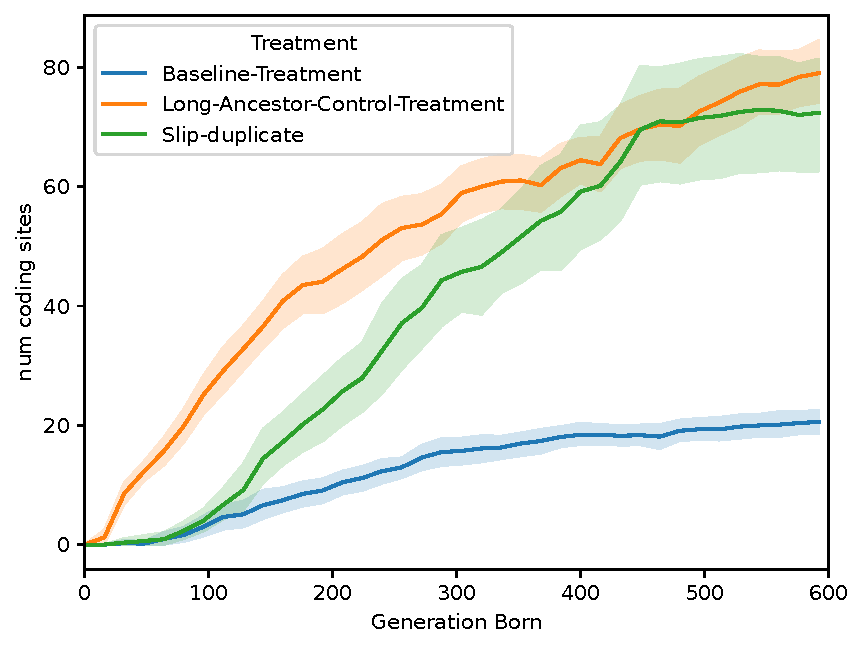
\includegraphics[width=\linewidth]{binder/binder/teeplots/hue=treatment+post=plt-xlim-0-600+viz=lineplot+x=generation-born+y=num-coding-sites+ext=.pdf}
    \caption{\footnotesize active coding sites}
    \label{fig:num-coding-sites:active}
    \end{subfigure}

    \begin{subfigure}{\linewidth}
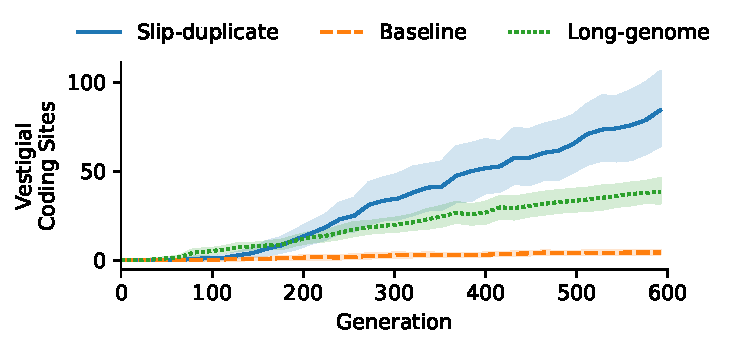
\includegraphics[width=\linewidth,clip, trim=0 0 0 0.8cm]{binder/binder/teeplots/hue=treatment+post=plt-xlim-0-600+viz=lineplot+x=generation-born+y=num-free-sites+ext=.pdf}
    \caption{\footnotesize vestigial coding sites}
    \label{fig:num-coding-sites:vestigial}
    \end{subfigure}
    \caption{
        \textbf{Gene duplication boosts accumulation of vestigial coding sites.}
        \footnotesize
        Generation-by-generation counts of coding sites over evolutionary history.
        Here, ``active'' coding sites refer to genome instructions determined through knockout to contribute to fitness with respect to self-copy viability or a rewarded phenotypic trait.
        As shown in panel \ref{fig:num-coding-sites:active}, gene duplication yields active coding site counts comparable to long-genome control.
        Vestigial coding site count, by contrast, reports the number of sites determined to have contributed to fitness in an ancestor, but are no longer active coding sites.
        As shown in panel \ref{fig:num-coding-sites:active}, vestigial coding site count under slip-duplication treatment outpace control treatments.
        Error bands give 95\% CI, bootstrapped over 30 replicates per treatment.
    }
    \label{fig:num-coding-sites}
\end{figure}


In a final set of analyses, we broadened our scope to assess consequences of gene duplication on genome architecture with respect to genome robustness \citep{lenski1999genome}.
We quantified robustness by counting the number of ``critical'' genome sites, where a single-site knockout disrupted replicator viability or adaptive phenotypic traits.%
\footnote{%
Although sufficiently representative for our purposes, limitations exist in detecting Avida genome functionality through single-site knockouts; such an approach can underestimate aspects of genome sequence complexity involving small effects or redundancy \citep{lenski1999genome,moreno2024cryptic}.
}

One conventional perspective on gene duplication is that copied genetic material reduces brittleness by introducing redundancy \citep{wagner1996genetic}.
To assess the relevance of this model within our study system, we performed slip-duplicate mutational assays to quantify the baseline effect of slip insertion mutations on robustness.
We applied our assay to lineages from slip duplication experiments, sampling one slip duplication per genome and measuring change in critical site counts between corresponding wildtype and mutated variants.

% @AML: Moved next line to discussion
% In line with evidence that duplication-associated redundancy can boost robustness \citep{Lynch2000}, fitness-neutral slip insertions did indeed tend to reduce the number of genome sites detectable as a single point of failure for performed tasks.
% https://github.com/chaynes2019/AvidaGeneDupe/blob/9fee1f13a8d31f25d1dd799c6a26f9b7fa617738/binder/indel-effect-nulldist.ipynb
On average, we found that fitness-neutral slip insertions decreased coding site count by 6.8 sites (bootstrapped 95\% CI 6.4 to 7.3; median 3\% of coding sites).
This effect was strongest in genomes with high complexity; for instance, neutral insertion mutations decrease coding site count by 9.2 and 8.3 sites on average in genomes that encode 4- and 5-component complexity tasks, respectively (bootstrapped 95\% CIs 8.5 to 9.9 and 7.2 to 9.3; median 3\% and 5\% of coding sites).
Supplementary Figure \ref{fig:nulldist} presents these results.

% https://github.com/chaynes2019/AvidaGeneDupe/blob/binder/binder/gain-mechanism.ipynb
To assess evolutionary consequences of redundancies introduced by slip-duplication, we next analyzed coding site accumulation within genomes over the course of evolution.
Counter to naive expectation, we found that the slip duplication treatment accrued fitness-critical sites at a generation-on-generation rate comparable to the long-genome baseline treatment; Mann-Whitney test, $U=361$, $p=0.19$).
Despite this similarity, however, when measurements were taken inclusive of vestigial coding sites (those which had \textit{previously} been fitness-critical earlier within a lineage), we found a significantly increased coding site count associated with the slip-duplicate treatment (Mann-Whitney test, $U=630$, $p<0.01$).
Figure \ref{fig:num-coding-sites} compares growth in active versus vestigial coding site counts for baseline, long-genome, and slip-duplication treatment.
% @AML: moved next line into discussion
% Within our study system, slip duplication appears to increase the net supply of coding material in the genome available to neutral processes, but not significantly affect accumulation of genetic brittleness.

% Indeed, in nature, large-scale genomic analyses have discovered cases where a strikingly high fraction of the genes in an organism show evidence of having arisen from gene duplications \citep{teichmann_structural_1998,Teichmann:2004cz}.
% Comparative studies have associated duplication events early in natural history with increases in genetic robustness and evolutionary innovation \citep{Wagner2008}.

% One possible explanation is that selective pressures are driving the two treatments to reach a similar number of critical sites, but slip duplication can duplicate and copy genome content in a manner that increases the copy count of previously coding sites relative to the number of critical sites.

\section{Discussion} \label{sec:discussion}

% -- Summary + key findings --
% @AML: Some of the discussion sections that I looked at (but not all) lead with a recap of authors' approach / questions.
%       - The recap can be nice for readers who jump around sections, but I'd be fine cutting it if we need the space or if folks feel that it's too redundant with the rest of the manuscript.
%      - Pretty much copied over the key findings from the cover letter
In this work, we used \textit{in silico} evolution experiments to investigate how gene duplication influences the evolution of biological complexity.
Specifically, we examined the hypothesis that gene duplication acts in shaping adaptive evolution of complex traits.
To conduct these experiments, we adapted a framework developed by Lenski et al. \citep{Lenski2003Evolutionary} to introduce adaptive potential for phenotypic traits across a well-defined spectrum of functional complexity (Figure \ref{fig:slip_mut_variants}).

Overall, our results support the premise that gene duplication can promote the \textit{de novo} evolution of adaptive traits.
Leveraging the unique tractability of our study system, we were able to explore these dynamics in greater detail, providing key insights into:
(1) sensitivity of potentiation effects to trait complexity,
(2) contributions of sequence information in duplicated material to adaptive outcomes, and
(3) a nuanced role of duplications in enhancing short-term robustness while predominantly promoting accumulation of vestigial coding material rather than neutral increases in complexity.

\subsection{Gene duplication facilitates adaptive evolution of complex traits}

While we find that gene duplication can facilitate adaptive evolution, we detect this effect only for phenotypic traits with greater functional complexity; adaptive evolution of simpler traits exhibits no benefit beyond the effect of increased genome size alone (Figure \ref{fig:adaptive-evolution-rate}).
Given the compositional nature of trait functionality within our study system \citep{Lenski2003Evolutionary}, this outcome would be consistent with a ``building block'' model of adaptation, where duplication facilitates discovery of novel medleys of existing components.

In broad strokes, adaptive significance of gene duplication within our study system aligns with existing findings across a wide variety of biological taxa and digital models that slip-duplication of genetic material can facilitate evolution of adaptive traits \citep{Koza:1995fr,Zhang:2003fw,Teichmann:2004cz}.
Indeed, a striking example of gene duplication potentiating novel adaptation comes from the Long-Term Evolution Experiment in \textit{E. coli} \citep{lenski1991longterm,Lenski2003phenotypic}, where a duplication in one population broadened expression of a key citrate transporter to aerobic conditions --- resulting in a seven-fold increase in carrying capacity within experimental conditions \citep{blount_genomic_2012}.
Among many other examples in nature \citep{zhang2002adaptive,gaines2009gene,perry2007diet,hittinger2007gene,benderoth2006positive,dulai1999evolution,Ogino2015}, such observations provide a basis for longstanding connections drawn between gene duplications and adaptive traits, dating as far back as \citet{ohno1970evolution}.

Present work, however, contrasts with recent directed evolution experiments investigating the effect of gene copy count on adaptation rate \citep{mihajlovic2025direct}.
This work finds no effect of gene copy count on phenotypic adaptation rate, comparing single- vs. dual-copy coGFP \textit{E. coli} strains under selection for increased fluorescence.
Several factors may explain this discrepancy, including our use of longer generational timescales and more naturalistic selection coefficients and mutational processes.
An contributing aspect may also be the opportunity for more open-ended, multi-gene composition of phenotypic traits in our study system.
Importantly, our work broadens the conversation by providing systematic and controlled experimental evidence supporting the role of gene duplication in adaptive evolution.
In particular, our findings suggest that the adaptive benefits of gene duplications may be especially important for the evolution of complex traits.
However, future studies will be necessary to determine whether similar constraints and patterns hold in natural systems, where additional mechanisms such as structured regulatory interactions may significantly influence trait evolution.

\subsection{Sequence information of duplications contributes to adaptive outcomes}

Our digital evolution study system allowed us to further disentangle which characteristics of gene duplications increase evolutionary potential by imposing variants of the slip mutation operator, isolating individual aspects of duplicative processes (Figure~\ref{fig:slip_mut_variants}).
We find that only duplications of existing genetic information --- either as-is or in a ``scrambled'' order --- provide adaptive benefit, with those preserving both content and order ultimately performing best.
In contrast, slip mutation variants that insert neutral or random genetic material provide no observable adaptive benefit over a baseline control (Figure~\ref{fig:results_panels}).
These results indicate that both the content and structure of duplicated genetic material contribute to facilitating adaptive evolution, beyond the impact of side effects such as an increase in genome size or mutational supply.
This finding is consistent with theoretical expectations that gene duplications generate both raw material and combinatorial novelty, enabling subfunctionalization and neofunctionalization \citep{ohno1970evolution,Lynch2000}.

Interestingly, unlike our long-genome control, we did not observe an adaptive benefit from the NOP-insert slip-duplication treatment (Figure~\ref{fig:results_panels}).
One possible explanation for this difference is selection against mutational load associated with increased genome length.
Indeed, in preliminary experiments we found that deleterious mutational load associated with larger genome size frequently drove extreme genome shrinkage, necessitating a lower bound on genome size.
As shown in Supplementary Figure~\ref{fig:ablation-site-counts}, we found genome size to grow significantly larger under full slip-duplication compared to NOP-insert slip-duplication --- by a factor of almost 4$\times$.
This pattern aligns with established theory that mechanistic factors such as dose effects or neutral accumulation of arbitrary interdependencies (e.g., ``complexity ratchet'' effects \citep{Liard2020,Soyer2006,Luke2011,gould1996full}) are necessary in ensuring preservation of new genome content \citep{Innan2010,Wagner1998,Tautz1992,Force1999,Bergthorsson2007}.

\subsection{Duplicated sites are potentiated for complex traits}

Through step-by-step analysis of lineage histories, we found that duplicated content was disproportionately likely to contribute to novel complex traits (Figure~\ref{fig:potentiation}).
An outsized fraction of coding sites for newly gained adaptive traits could be traced back to duplicated regions, and a substantial fraction of gain-of-function mutations (41 of 174 along analyzed lineages) directly coincided with slip duplications.
Thus, the adaptive characteristics of slip duplication observed in our system likely result from a combination of direct facilitation and potentiation of subsequent neo-functionalization.
This pattern concords with large-scale analyses of biological genomes, which have  revealed that a high fraction of genes show evidence of having arisen from duplications \citep{teichmann_structural_1998,Teichmann:2004cz}.
As such, our results support long-standing hypotheses about the role of gene duplications in evolutionary innovation and highlight the mechanistic basis for the observed increase in evolvability, particularly for traits requiring multiple interacting components.

\subsection{Genome length drives genetic complexity}

Consistent with evidence that duplication-associated redundancy can boost robustness \citep{Lynch2000}, we found that slip insertions with neutral fitness effects tended to reduce the number of genome sites detectable as a single point of failure for metabolic tasks or reproductive viability (Supplemental Figure \ref{fig:nulldist}).
Within evolutionary trials in our study system, slip duplication appears to increase the net supply of coding material in the genome available to neutral processes, but does not significantly affect accumulation of genetic brittleness (Figure \ref{fig:num-coding-sites}).
One possible explanation is that, despite slip duplication boosting redundancy in the short term, mutational erosion and selective pressures against mutational fragility drive both the slip-duplication and long-genome treatments to converge on a similar number of critical sites.
On the other hand, observed proliferation of vestigial coding material by gene duplications aligns with adaptive potentiation effects discussed earlier.
Given that comparative studies have linked ancient duplication events with subsequent gains in genetic robustness and evolutionary innovation \citep{Wagner2008}, these findings suggest directions for future experimental work investigating how such dynamics unfold over extended timescales to shed light on possible connections to larger-scale evolutionary patterns.
